\section{Identifying Causality: Experiments vs Observational Studies}

Many studies are carried out to examine whether two variables (called explanatory and response variables) are related to each other.

Such studies can be either of two types

\textbf{Observational study:} The investigator merely observes whether the two variables vary together. The big thing here is that no attempt is made to induce changes in the response variable.

\textbf{Experiment:} Treatments are imposed on individuals. A deliberate attempt is made to induce change in the response variable.

An observational study on its own CANNOT establish cause and effect. This is because observational studies suffer from the possible presence of variables whose effects on the response are confounded the effect (if any) of the explanatory variable.

\subsection{Exercise}

An observational study shows that people who eat foods reach in antioxidants like fruits and vegetables have lower rates of colon cancer than those who dont eat those foods. 

\textbf{Question:} Can we conclude that eating such food reduces the risk of colon cancer?

\textbf{Answer:} No because this is an observational study. 

\textbf{Confounding variables:} Health consciousness (e.g. exercise, access to medical care, amount of drinking/smoking, income, etc.)

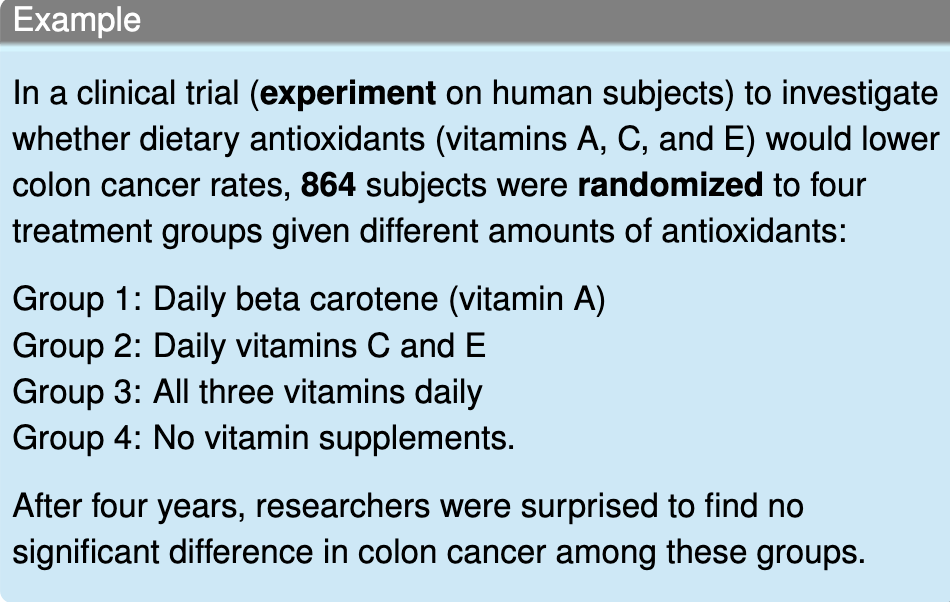
\includegraphics[scale=0.5]{experiment_example}
